%% KinoVLA --- ICRA conference paper
%% Sections drafted in this file: Abstract, Introduction, Related Work.
%% Compile: pdflatex main && bibtex main && pdflatex main && pdflatex main
%% Requires the IEEEtran document class and IEEEtran.bst (ships with most TeX
%% distributions; otherwise: https://www.ctan.org/pkg/ieeetran).
%%
%% The paper is set up for DOUBLE-BLIND review (anonymous author block). For a
%% camera-ready version, replace the anonymous block with the real authors and
%% comment out the \def\isanonymous line below.
\def\isanonymous{1}

\documentclass[conference]{IEEEtran}
\IEEEoverridecommandlockouts

\usepackage{cite}
\usepackage{amsmath,amssymb,amsfonts}
\usepackage{graphicx}
\usepackage{textcomp}
\usepackage{xcolor}
\usepackage{booktabs}
\usepackage[hidelinks]{hyperref}
\usepackage{url}
\usepackage{tikz}
\usetikzlibrary{positioning, arrows.meta, calc}

% Sub-millisecond, capture point, and other inline math are used in the body.
\newcommand{\kinovla}{Kino-VLA}
\newcommand{\kinofail}{Kino-Fail}
\newcommand{\kinotokens}{Kino-Tokens}

\begin{document}

\title{\kinovla{}: Closed-Loop Embodied Reflection for\\
Semantic Failure Recovery in Quadrupedal Locomotion}

\ifdefined\isanonymous
  \author{\IEEEauthorblockN{Anonymous Author(s)}
  \IEEEauthorblockA{Paper under double-blind review\\
  Affiliation and contact details omitted for anonymity}}
\else
  \author{\IEEEauthorblockN{First Author\IEEEauthorrefmark{1},
  Second Author\IEEEauthorrefmark{1}, and Third Author\IEEEauthorrefmark{1}}
  \IEEEauthorblockA{\IEEEauthorrefmark{1}Institution Name\\
  \texttt{\{first, second, third\}@institution.edu}}}
\fi

\maketitle

\begin{abstract}
Learned controllers and rapid motor adaptation let legged robots reject a wide
range of disturbances by reacting continuously to proprioceptive history. A
distinct class of physical failures, however, cannot be recovered this way:
escaping an elastic tether requires backing off rather than applying more
torque, and a foot held by an adhesive trap is proprioceptively
indistinguishable from one sinking into mud, yet the two demand opposite
recoveries. Such failures require discrete, topological, strategy-level
decisions that lie outside the hypothesis space of any continuous adaptive
controller. We present \kinovla{}, a closed-loop embodied-reflection framework
that couples high-frequency dynamics sensing with a vision-language recovery
planner for a quadrupedal robot. Recovery is organized into five layers: a
\mbox{1\,kHz} monitor-and-reflex loop that keeps the robot upright while
reasoning proceeds; a \kinotokens{} extractor that distills \mbox{1\,kHz}
proprioception into the language model's embedding space under privileged-physics
supervision; a vision-language planner that performs causal failure attribution,
selects from an expanded recovery-primitive library, and maintains a persistent
semantic traversability map; and a control-barrier-function safety shield that
projects every proposed primitive onto a provably safe set, with a
forward-invariance guarantee that, under a reduced-order model, the closed loop
never leaves that set regardless of what the language model outputs. We further contribute
\kinofail{}, a benchmark of eleven continuously parameterized failure operators
with privileged ground truth and constructively matched attribution-ambiguity
pairs, and a privileged-grounded hindsight chain-of-thought data pipeline whose
truth-consistency filter rejects any annotation contradicted by simulator
physics. In high-fidelity simulation on a physically simulated Unitree Go2, the
trained planner attains \mbox{0.97} attribution accuracy on
semantic-intervention failures, against \mbox{0.24} for a tuned rule-based state
machine, while the safety shield solves in under \mbox{0.2\,ms}.
\end{abstract}

\begin{IEEEkeywords}
Legged robots, vision-language-action models, failure recovery, control barrier
functions, embodied AI, safe learning, quadrupedal locomotion.
\end{IEEEkeywords}

%% ===================================================================
\begin{figure*}[t]
\centering
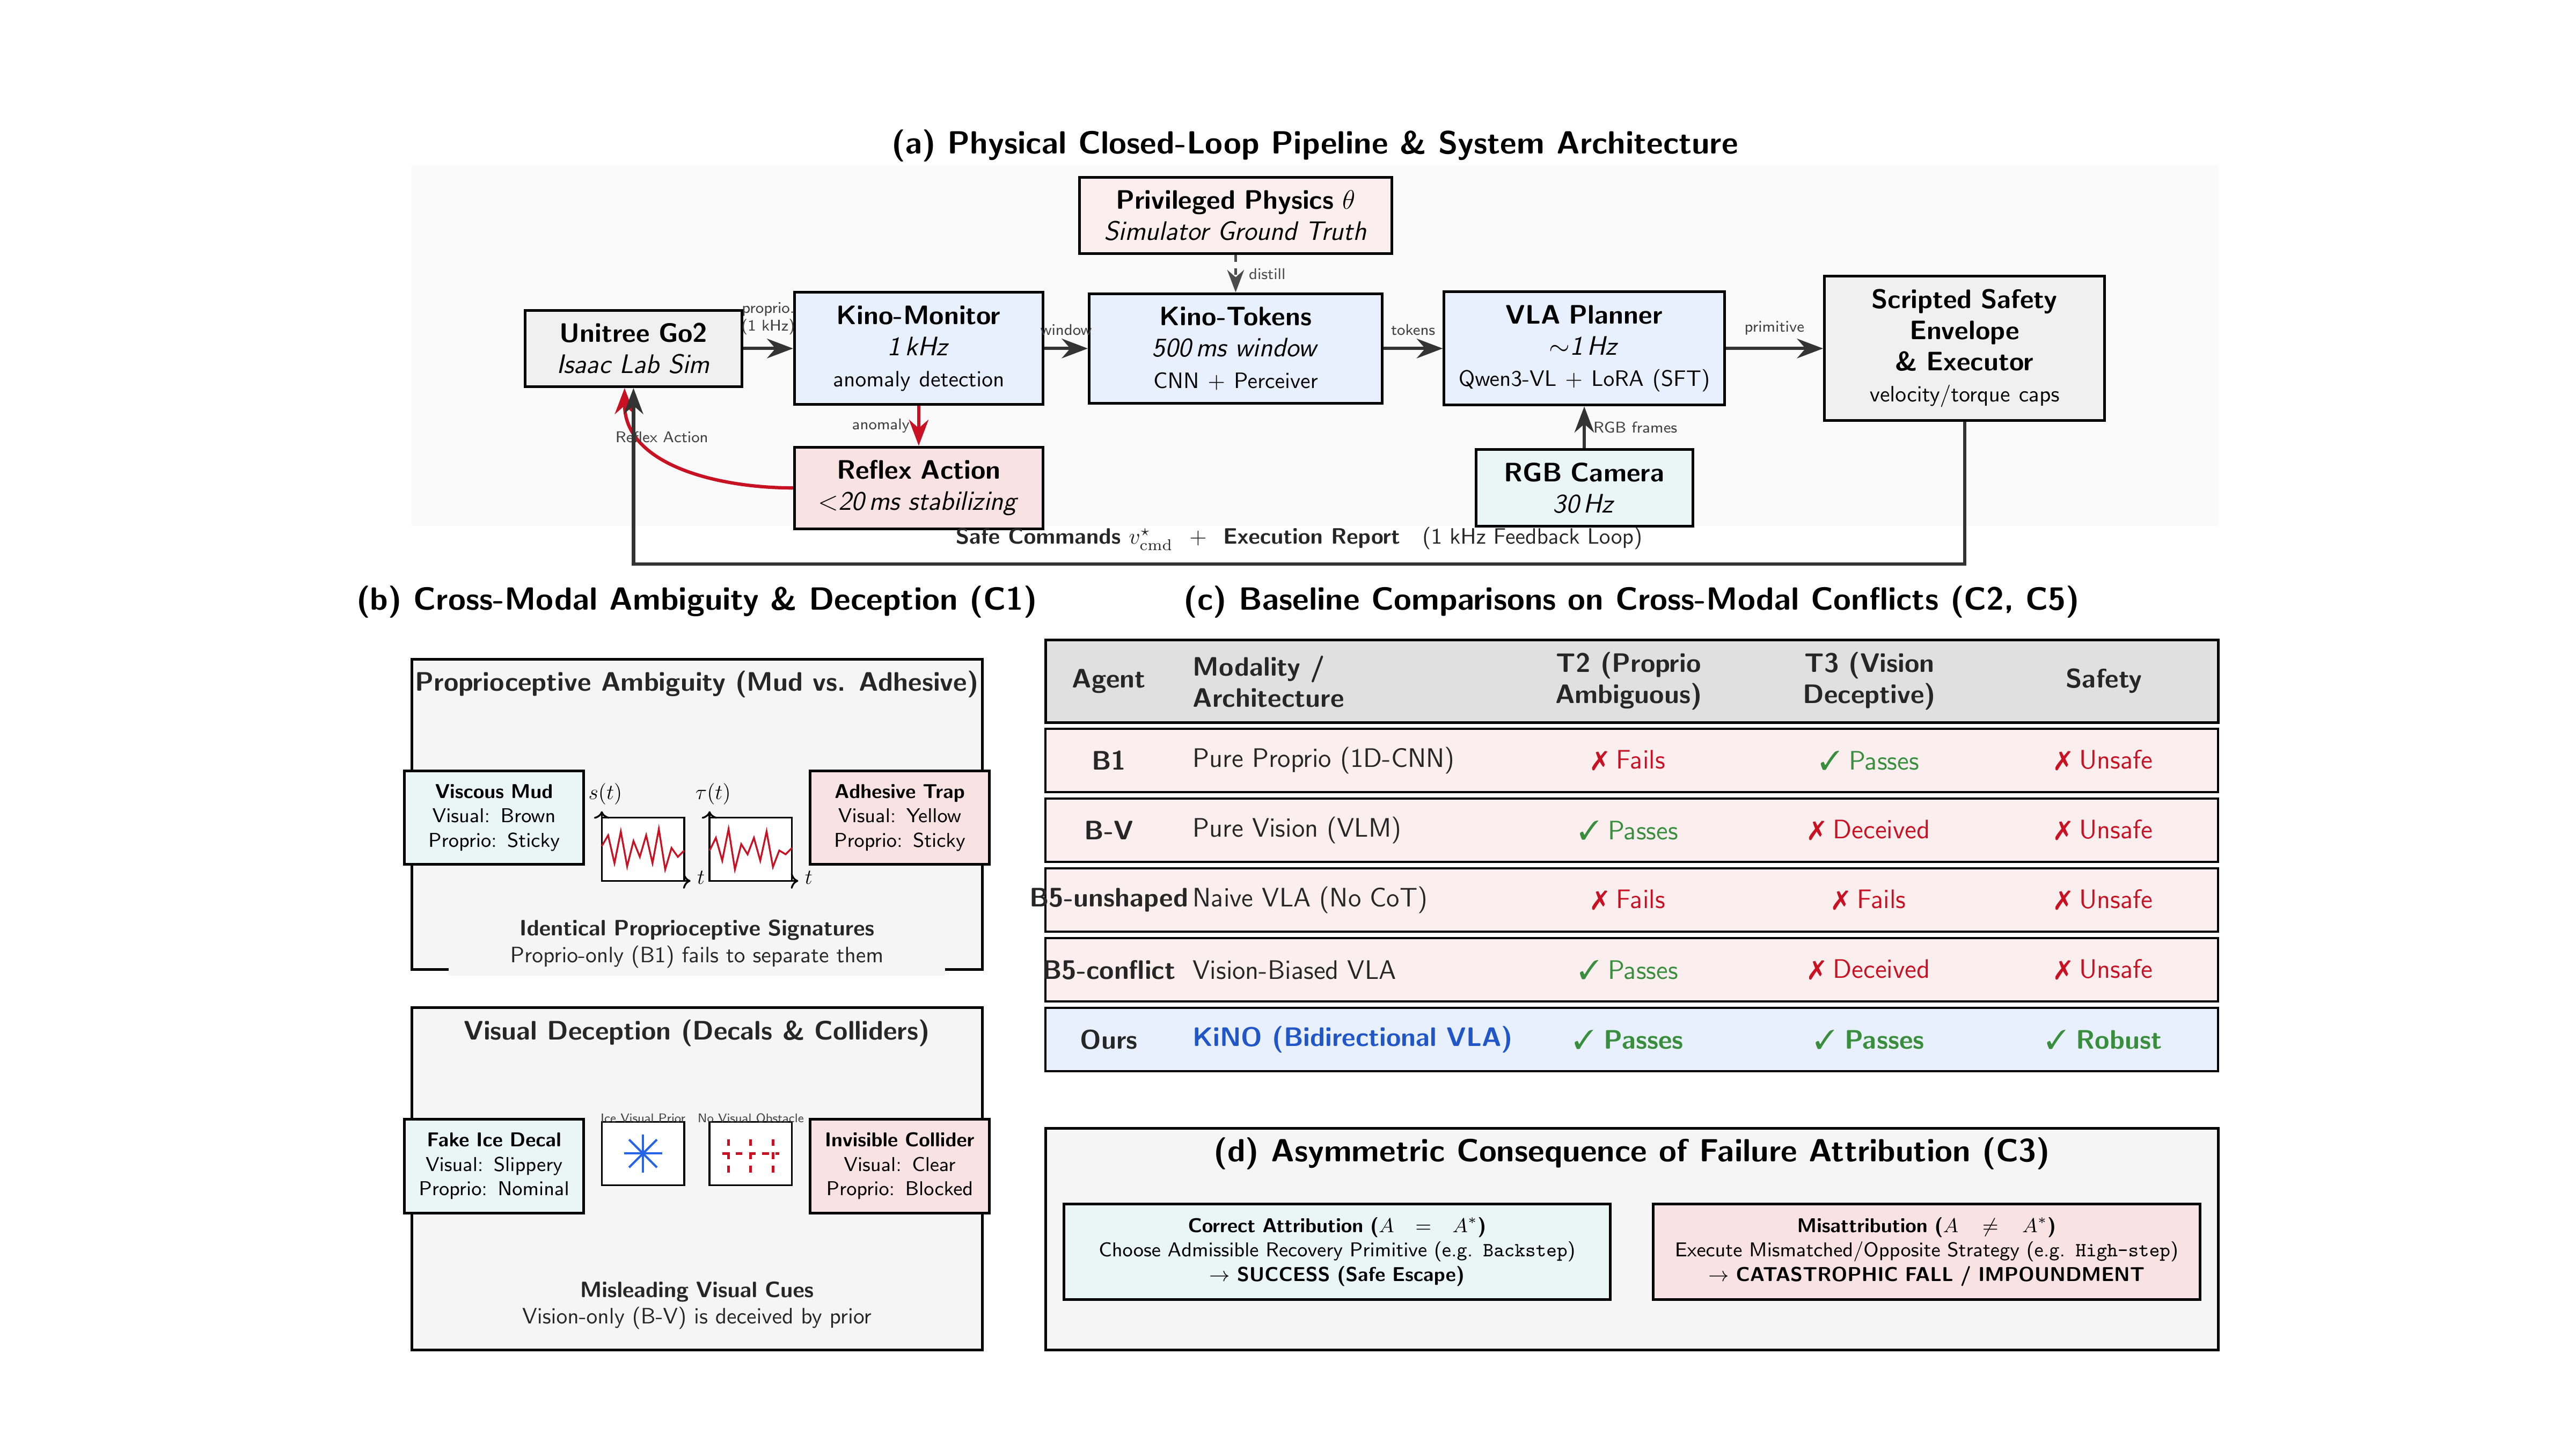
\includegraphics[width=\textwidth]{fig1_framework.png}
\iffalse  %% original TikZ source preserved below; figure is now rendered as fig1_system.png
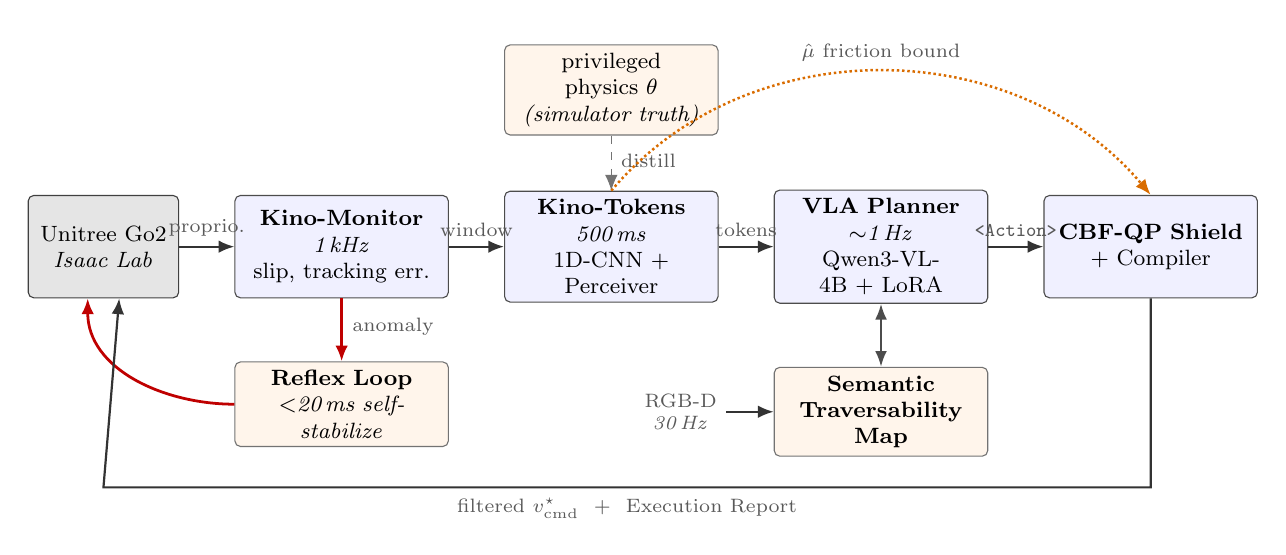
\begin{tikzpicture}[
  font=\footnotesize,
  layer/.style={rectangle, rounded corners=2pt, draw=black!70, fill=blue!6,
                align=center, minimum height=13mm, text width=25mm, inner sep=3pt},
  plant/.style={rectangle, rounded corners=2pt, draw=black!75, fill=black!10,
                align=center, minimum height=13mm, text width=17mm, inner sep=3pt},
  aux/.style={rectangle, rounded corners=2pt, draw=black!55, fill=orange!8,
              align=center, minimum height=10mm, text width=25mm, inner sep=3pt},
  lab/.style={align=center, font=\scriptsize, text=black!65},
  fwd/.style={-{Latex[length=2mm,width=1.6mm]}, thick, black!80},
  fast/.style={-{Latex[length=2mm,width=1.6mm]}, line width=1pt, red!75!black},
  distill/.style={-{Latex[length=2mm,width=1.6mm]}, dashed, black!55},
  couple/.style={-{Latex[length=2mm,width=1.6mm]}, densely dotted, line width=0.9pt, orange!85!black},
]
% main forward pipeline
\node[plant] (robot) {Unitree Go2\\\textit{Isaac Lab}};
\node[layer, right=7mm of robot] (mon) {\textbf{Kino-Monitor}\\\textit{1\,kHz}\\slip, tracking err.};
\node[layer, right=7mm of mon] (tok) {\textbf{Kino-Tokens}\\\textit{500\,ms}\\1D-CNN $+$ Perceiver};
\node[layer, right=7mm of tok] (vla) {\textbf{VLA Planner}\\\textit{$\sim$1\,Hz}\\Qwen3-VL-4B $+$ LoRA};
\node[layer, right=7mm of vla] (cbf) {\textbf{CBF-QP Shield}\\$+$ Compiler};
\draw[fwd] (robot) -- node[lab,above]{proprio.} (mon);
\draw[fwd] (mon) -- node[lab,above]{window} (tok);
\draw[fwd] (tok) -- node[lab,above]{tokens} (vla);
\draw[fwd] (vla) -- node[lab,above]{\texttt{<Action>}} (cbf);
% privileged distillation (training-time supervision)
\node[aux, above=7mm of tok] (theta) {privileged physics $\theta$\\\textit{(simulator truth)}};
\draw[distill] (theta) -- node[lab,right,pos=0.45]{distill} (tok);
% mu-hat coupling, over the top
\draw[couple] (tok.north) to[out=50,in=130] node[lab,above]{$\hat\mu$ friction bound} (cbf.north);
% reflex fast loop
\node[aux, below=8mm of mon] (reflex) {\textbf{Reflex Loop}\\\textit{$<$20\,ms self-stabilize}};
\draw[fast] (mon) -- node[lab,right,pos=0.45]{anomaly} (reflex);
\draw[fast] (reflex.west) to[out=180,in=-90] ([xshift=-2mm]robot.south);
% semantic map + RGB-D
\node[aux, below=8mm of vla] (map) {\textbf{Semantic}\\\textbf{Traversability Map}};
\draw[{Latex[length=2mm]}-{Latex[length=2mm]}, thick, black!70] (vla) -- (map);
\node[lab, left=6mm of map] (rgbd) {RGB-D\\\textit{30\,Hz}};
\draw[fwd] (rgbd) -- (map);
% big feedback loop: cbf -> robot
\draw[fwd] (cbf.south) -- ([yshift=-24mm]cbf.south)
  -- node[lab,below]{filtered $v_{\mathrm{cmd}}^{\star}$ \ $+$ \ Execution Report} ([yshift=-24mm]robot.south)
  -- ([xshift=2mm]robot.south);
\end{tikzpicture}
\fi
\caption{\textbf{The \kinovla{} framework.} \textbf{(a) Recoverability dichotomy.}
A-class failures (uniform low friction, a static load, a viscous floor) are
recovered by continuous adaptation; B-class failures need a strategy-level
decision. An adhesive trap (O4) and viscous mud (O2) produce \emph{identical}
proprioception---resistance, slip, and torque coincide---yet demand opposite
recoveries (back off vs.\ switch gait), so only vision can decide. \textbf{(b)
\kinofail{} benchmark.} Eleven parameterized failure operators on four mechanism
axes, each exposing a privileged ground-truth parameter $\theta$ (friction,
payload, effort, support); three constructively matched ambiguity pairs
(O1$\leftrightarrow$O3, O2$\leftrightarrow$O4, O5$\leftrightarrow$O10) on which
proprioception coincides; and five evaluation suites (Cal, Sem, Comp, Bound, OOD).
\textbf{(c) Closed loop} on a physically simulated Unitree Go2. A \mbox{1\,kHz}
Kino-Monitor and a millisecond reflex keep the robot upright; a \kinotokens{}
extractor distills a \mbox{500\,ms} proprioceptive window into the planner under
privileged-physics supervision; the \mbox{$\sim$1\,Hz} VLA planner---trained on the
truth-filtered hindsight chain-of-thought data from (b)---attributes the failure,
emits one recovery primitive, and reads and writes a persistent semantic
traversability map, while the CBF-QP shield projects every primitive onto a
provably safe set ($<$\mbox{0.2\,ms}) before it is compiled to a velocity command.}
\label{fig:system}
\end{figure*}

%% ===================================================================
\section{Introduction}
\label{sec:intro}

Reinforcement learning has made quadrupedal locomotion remarkably robust.
Policies trained in simulation with domain randomization, and augmented with
online motor adaptation, cross rubble, mud, and ice and reject pushes that would
topple a hand-tuned controller~\cite{lee2020learning,miki2022learning,kumar2021rma,nahrendra2023dreamwaq}.
This robustness rests on continuous reaction: from a window of proprioceptive
history the controller implicitly infers the local dynamics (friction, payload,
terrain compliance) and adjusts its gait within a continuous parameter
space~\cite{kumar2021rma}. For a broad family of disturbances this is the
correct response, and we claim no improvement on it.

A separate family of failures defeats continuous reaction. A leg caught by an
elastic tether is the canonical case: an adaptive controller raises torque to
hold its commanded velocity, the tether stores that energy like a drawn bow, and
the accumulated load eventually flings the robot off balance, so the safe action
is the counter-intuitive one of backing off. Sudden resistance at a foot is a
second case: if the cause is an adhesive trap the robot must step back, label the
patch untraversable, and route around it, whereas if the cause is mud it must
raise its gait and drive through. The recoveries are opposite, yet the two causes
can be tuned to produce identical proprioceptive signatures, matched
tangential-resistance curves, slip distributions, and torque spectra, so a
controller reading proprioception alone cannot, even in principle, tell them
apart.

We make this structure explicit as a \emph{recoverability dichotomy}. A-class
failures (uniform low friction, a static load offset, a mildly viscous floor) are
recoverable by continuous adaptation, and an adaptive controller should handle
them as well as any semantic system does. B-class failures require a discrete,
topological, or strategy-level decision (back off, declare an entire region
impassable, or abandon a torque-saturated task and request help), and an
incorrect causal attribution produces the wrong, frequently opposite, recovery.
What sets B-class failures apart is that the decision turns on a cause
proprioception cannot resolve but vision can, such as the yellow sheen of a glue
board against the brown of mud. These decisions lie outside the hypothesis space
of any continuous adaptive controller and inside that of a semantic one. The
scientific question we pose and answer empirically follows: which physical
failures are recoverable by low-level adaptation, and which require semantic
intervention?

Existing learning systems leave the B-class gap open. End-to-end
vision-language-action models map observations to actions open-loop and at low
frequency, without a force-feedback channel, and commit to a planned action
through a developing
failure~\cite{brohan2023rt2,kim2024openvla,octo2024,driess2023palme}. Visually
closed-loop planners react to RGB at camera rate~\cite{bu2024clover,zhi2024comerobot}
and stay blind to a friction collapse or an actuator saturation until it has
produced an overt visual symptom. Legged navigation models built on language
backbones treat locomotion as a one-way black-box
skill~\cite{cheng2024navila,mei2024quadrupedgpt,wu2024doggybot}: the planner
issues velocity or waypoint commands but receives no upward report that the body
is slipping or pinned. Closest to our aim, failure-reasoning systems such as
REFLECT~\cite{liu2023reflect} and AHA~\cite{duan2025aha} summarize multimodal
experience to explain and correct manipulation failures, but they attribute after
the fact from low-frequency vision, address fixed-base manipulators rather than an
underactuated floating-base robot, and inject conclusions as discrete text; on a
legged platform they additionally lack the millisecond reflex that would keep the
robot upright during the roughly one second of language-model inference.

We present \kinovla{}, a closed-loop embodied-reflection framework that supplies
the missing upward channel from \mbox{1\,kHz} dynamics to a semantic planner and
the missing downward guarantee that the planner cannot destabilize the robot.
\kinovla{} organizes recovery into five layers (Fig.~\ref{fig:system}). A \mbox{1\,kHz} Kino-Monitor
computes slip and tracking-error statistics and triggers a reflex loop that
stabilizes the body (brake, stiffen, lower the center of mass) within
milliseconds, bypassing the language model. A \kinotokens{} extractor compresses
a \mbox{500\,ms} proprioceptive window with a 1D convolutional network and a
Perceiver Resampler~\cite{jaegle2021perceiver,alayrac2022flamingo} into
fixed-length tokens projected into the language model's embedding space; the
latent is supervised by distillation against privileged simulator
physics~\cite{chen2020cheating,kumar2021rma}, with an auxiliary physics-text
contrastive objective~\cite{oord2018cpc}, so the tokens carry interpretable
physical meaning and a calibrated out-of-distribution score. A roughly
\mbox{1\,Hz} planner, a LoRA-adapted~\cite{hu2022lora} vision-language
model~\cite{bai2025qwen3vl,wang2024qwen2vl}, fuses vision, text, and
\kinotokens{} to attribute the failure causally, selects a single primitive from
an expanded recovery library, and maintains a persistent semantic traversability
map onto which physical evidence is written. A control-barrier-function (CBF)
safety shield and primitive compiler then project every proposed primitive onto a
provably safe set before execution. Two ideas carry the design. First,
\emph{the language model proposes, the barrier function disposes}: a CBF quadratic
program minimally edits each primitive so the capture point cannot leave a
contracted support polygon, which yields a forward-invariance guarantee, under a
reduced-order model, that the closed loop remains in its safe set whatever the
language model outputs~\cite{ames2017control,pratt2006capture}. Second, privileged
physics grounds both the latent and the training data, replacing an unanchored
black box with quantities the simulator can verify.

To study the dichotomy we introduce \kinofail{}, a benchmark of eleven
continuously parameterized failure operators across four simulator mechanism
axes, each exposing its parameter vector as privileged ground truth. Three
operator pairs are constructed so their proprioceptive statistics coincide,
making a proprioception-only baseline fail on them by design, and a dedicated
suite sweeps an operator's parameter across the A/B frontier, turning the
question of when semantic intervention becomes necessary into a measurable curve.
To train the planner we build a privileged-grounded hindsight
chain-of-thought~\cite{wei2022chain} pipeline whose central component is an
automated truth-consistency filter: an oracle annotation is kept only if its
physical attribution matches the privileged parameters and its chosen primitive
lies in the feasible recovery set, which converts ``the oracle guessed'' into
``physically grounded.'' The planner is then trained in two stages, supervised
fine-tuning on the filtered data followed by an embodied preference-optimization
stage~\cite{rafailov2023dpo} that scores rollouts by their physical outcome.

We implement and evaluate \kinovla{} in high-fidelity simulation on a physically
simulated Unitree Go2 in Isaac Lab~\cite{makoviychuk2021isaacgym,mittal2023orbit}.
On held-out semantic-intervention failures the trained planner attains an
attribution accuracy of \mbox{0.97}, against \mbox{0.24} for a tuned rule-based
state machine, and every sampled output parses against the action schema; the
safety shield solves its quadratic program in under \mbox{0.2\,ms} at the
ninety-ninth percentile; and the privileged-distillation extractor regresses
friction, payload, actuator effort, and support state to within per-operator
tolerances. Sim-to-real transfer is treated at the level of design (an
actuator-network model and contact-signal randomization) and left to future
hardware studies.

\noindent This paper makes the following contributions.
\begin{itemize}
  \item We formalize the \emph{recoverability dichotomy} as a falsifiable
  question and instantiate it as \kinofail{}, a parameterized failure-operator
  benchmark with privileged ground truth and three constructively matched
  attribution-ambiguity pairs that render proprioception-only recovery provably
  insufficient.
  \item We cast the safety layer as a CBF quadratic program that arbitrates the
  unconstrained output of a language model, with a forward-invariance guarantee in
  a capture-point reduced-order model and an explicit dual-rate latency budget
  under which the reflex loop keeps the robot alive while the planner reasons.
  \item We ground the cross-frequency interface in privileged physics: a distilled
  \kinotokens{} latent with a calibrated out-of-distribution score, and a hindsight
  chain-of-thought pipeline whose truth-consistency filter rejects physically
  inconsistent annotations.
  \item We show, in simulation, that the resulting planner attributes and recovers
  from semantic-intervention failures where a tuned rule-based baseline cannot,
  evidence for the irreplaceability of vision-grounded reasoning on the B-class
  subspace.
\end{itemize}

%% ===================================================================
\section{Related Work}
\label{sec:related}

\subsection{Learned legged locomotion and online adaptation}
Model-free reinforcement learning produces quadrupedal controllers that walk over
challenging terrain~\cite{lee2020learning,miki2022learning} and adapt online to
unmodeled dynamics by encoding proprioceptive history into a latent that drives
the policy~\cite{kumar2021rma,nahrendra2023dreamwaq}. These controllers are
trained at scale with massively parallel simulation~\cite{rudin2022learning,makoviychuk2021isaacgym,mittal2023orbit}
and transferred to hardware with actuator-network models of motor and gearbox
nonlinearity~\cite{hwangbo2019learning}. Most use teacher-student privileged
distillation, in which a student trained on onboard observations regresses a
teacher's access to privileged simulator state~\cite{chen2020cheating,lee2020learning};
we reuse exactly this mechanism for \kinotokens{}. The boundary is deliberate. These
methods encode dynamics to drive a continuous control policy, and we make no claim
to improve their adaptation. We distill the same privileged signal into a
\emph{semantic} embedding that supports discrete decisions, and we target the
B-class subspace where continuous adaptation is insufficient by construction rather
than merely suboptimal.

\subsection{Vision-language-action models and embodied foundation models}
Large multimodal models have been adapted into robot policies that map language
and pixels to actions~\cite{brohan2023rt1,brohan2023rt2,kim2024openvla,octo2024,driess2023palme,li2024roboflamingo,black2024pi0},
and into high-level reasoners that sequence skills through language~\cite{ahn2022saycan,liang2023codeaspolicies,huang2022inner}.
Legged variants extend this recipe to navigation~\cite{cheng2024navila,mei2024quadrupedgpt,wu2024doggybot},
and visually closed-loop systems re-plan from RGB observations as a task
unfolds~\cite{bu2024clover,zhi2024comerobot}. In all of these, action is generated
open-loop or closed only on vision at camera rate, and on legged platforms
locomotion is invoked as a black-box skill that returns no dynamics feedback.
\kinovla{} adds a \mbox{1\,kHz} proprioceptive channel into the planner and a
barrier-certified compiler beneath it, so the planner both sees the failure in the
dynamics and cannot issue an action that destabilizes the body.

\subsection{Failure detection, attribution, and language-model recovery}
A growing line of work uses language and vision models to explain and correct
robot failures. REFLECT~\cite{liu2023reflect} summarizes multimodal robot
experience into a hierarchical trace for failure explanation, AHA~\cite{duan2025aha}
trains a vision-language model to detect and reason over manipulation failures,
and DoReMi~\cite{guo2024doremi} detects and recovers from plan-execution
misalignment. In parallel, classical legged-robot pipelines detect slip and
anomalies from proprioception~\cite{yan2025slip}, and introspective perception
predicts when a vision system will fail~\cite{daftry2016introspective}. The
distinctions are several. Attribution in the language-model line is performed after
the fact, from low-frequency vision or audio, on fixed-base manipulators, and is
injected as discrete text; classical legged anomaly detection stops at raising an
alarm. \kinovla{} attributes \emph{online}, during a reflex-maintained safe
interval, from a \mbox{1\,kHz} dynamics channel, and closes the loop through an
expanded recovery-primitive library and a persistent map rather than terminating
at an explanation or an alarm.

\subsection{Safe control and safety filters}
Control barrier functions provide quadratic-program safety filters with forward-invariance
guarantees~\cite{ames2017control,ames2019control}, and legged balance has long been
analyzed through reduced-order capture-point~\cite{pratt2006capture} and divergent-component-of-motion~\cite{englsberger2015three}
models built on the linear inverted pendulum and zero-moment-point
formulation~\cite{kajita2003biped}. Recent work layers barrier functions with model
predictive control for legged robots~\cite{grandia2021multi}, certifies learning-based
controllers with predictive safety filters~\cite{wabersich2018linear}, and surveys
the broader safe-learning program~\cite{brunke2022safe}. These methods certify a
\emph{known} controller against bounded disturbances. We instead place the CBF
quadratic program downstream of an unconstrained, potentially hallucinated
language-model output and project discrete recovery primitives onto a capture-point
safe set, which addresses formal safety for language-model-in-the-loop legged
control.

\subsection{Semantic maps and open-vocabulary perception for navigation}
Open-vocabulary scene representations build navigable maps by grounding vision into
3D with CLIP~\cite{radford2021clip} and SAM~\cite{kirillov2023sam} features~\cite{huang2023vlmaps,huang2023voxposer,chen2023nlmap},
and self-supervised traversability estimation learns terrain costs from
experience~\cite{frey2023wvn}. These approaches write traversability from vision
(vision $\rightarrow$ map). \kinovla{} inverts the direction: a physical failure
rewrites the visually derived label of its 3D region and propagates the correction
across visually homogeneous neighbors (physics $\rightarrow$ map), so that stepping
through a single broken patch of thin ice condemns the entire visually uniform
sheet.

%% ===================================================================
\section{The \kinovla{} System}
\label{sec:method}

\subsection{Overview}
\kinovla{} closes the loop from a \mbox{1\,kHz} dynamics stream to a roughly
\mbox{1\,Hz} semantic planner and back, in five layers running at three rates. A
\emph{Kino-Monitor} reads proprioception at \mbox{1\,kHz} and raises an anomaly
flag; a \emph{reflex loop} stabilizes the body within milliseconds; a
\emph{\kinotokens{} extractor} compresses a \mbox{500\,ms} dynamics window into
the planner's embedding space; a \emph{VLA recovery planner} attributes the
failure, selects a recovery primitive, and updates a semantic map; and a
\emph{CBF safety shield} with a primitive compiler runs at \mbox{500\,Hz}--\mbox{1\,kHz}.
The dual-rate design rests on the latency budget in Table~\ref{tab:latency}: the
reflex holds the state inside the safe set for a dwell time that covers the
planner's inference latency, while the shield guarantees that whatever the planner
eventually outputs cannot push the state out of the safe set. The reflex and the
shield together make the system safe in the A-class regime; the planner supplies
the semantic decision the B-class regime requires.

\begin{table}[t]
\centering
\caption{End-to-end latency budget of the dual-rate loop.}
\label{tab:latency}
\begin{tabular}{lr}
\toprule
Stage & Budget \\
\midrule
Anomaly $\rightarrow$ Kino-Monitor detection & $<5$\,ms \\
Reflex stabilization & $<20$\,ms \\
Kino-Token window fill & $500$\,ms \\
VLA inference & $\sim 1$\,s \\
CBF arbitration $+$ primitive compile & $<10$\,ms \\
\bottomrule
\end{tabular}
\end{table}

\subsection{Kino-Tokens: privileged-physics distillation}
The Kino-Monitor computes, at \mbox{1\,kHz}, a slip score and a velocity-tracking
error from onboard proprioception (joint torques estimated from motor current,
joint angles, IMU attitude). Crossing calibrated thresholds arms the reflex loop,
which applies a damping stand, a wider stance, and a lower center of mass without
invoking the planner, and gates the extractor on.

A \mbox{500\,ms} sliding window of proprioception is encoded by a 1D convolutional
network, which captures local transients, followed by a Perceiver
Resampler~\cite{jaegle2021perceiver,alayrac2022flamingo} that cross-attends the
window into fixed-length tokens $z$. The latent is supervised primarily by
distillation against privileged simulator physics, in the teacher-student style of
privileged learning~\cite{chen2020cheating,kumar2021rma}: a regression head $g$
predicts the privileged parameter vector $\theta$ (true friction $\mu$, contact
stiffness, payload mass, actuator effort limit) under a Huber loss
$\mathcal{L}_\theta = \mathrm{Huber}(g(z),\theta)$, with an auxiliary
InfoNCE~\cite{oord2018cpc} objective aligning $z$ to text. Privileged supervision
buys three properties: the latent is physically interpretable, out-of-distribution
detection becomes the \emph{measurable} residual of the $\theta$ prediction rather
than an abstract notion of manifold departure, and the same residual grounds the
data filter of Sec.~\ref{subsec:training}. A Kino-Projector multilayer perceptron
maps $z$ into the vision-language model's embedding space as soft tokens, and
anomaly-gated injection zeroes their weight at steady state, waking the channel
only on an alarm. The online estimate $\hat\mu$ is forwarded to the shield,
coupling perception to safety.

\subsection{Recovery planner and semantic traversability map}
The planner is a pretrained vision-language model (Qwen3-VL-4B~\cite{bai2025qwen3vl},
the successor to Qwen2-VL~\cite{wang2024qwen2vl}) adapted with
LoRA~\cite{hu2022lora}. At each step it consumes recent RGB frames, a textual
context (task, history, a crop of the current map, and any rejection codes from the
shield), and the \kinotokens{} as soft tokens; a text route that serializes the
physics summary into words replaces the soft tokens as an ablation arm. The planner
emits a structured response, a \texttt{<Thought>} chain of
reasoning~\cite{wei2022chain} followed by a \texttt{<Action>} that names one
primitive and its parameters. A schema-validating parser admits only well-formed
atomic actions, so no malformed command reaches the compiler.

The primitive library spans the locomotion policy's command space:
\texttt{Backstep}, \texttt{Replan\_Waypoint} (a 2D pixel goal back-projected to a 3D
waypoint), \texttt{Switch\_Gait}, \texttt{Adjust\_Posture}, \texttt{Set\_Constraint},
\texttt{Update\_Topology}, and \texttt{Hold\_and\_Request}. The
attribution-to-recovery mapping is many-to-many by design: identical proprioception
can demand opposite primitives, so a correct recovery depends on a vision-grounded
causal attribution that a controller over proprioception cannot make.

The semantic traversability map persists topological memory across viewpoints.
Open-vocabulary segmentation with CLIP~\cite{radford2021clip} and
SAM~\cite{kirillov2023sam} features partitions RGB into regions, and RGB-D depth
back-projection lifts them to 3D regions in the odometry frame, in the spirit of
language-grounded maps~\cite{huang2023vlmaps,chen2023nlmap} but driven in the
opposite direction. A visual prior seeds traversability; when a physical failure
occurs, the \kinotokens{} attribution overwrites the corresponding region's
costmap label as high-confidence evidence, and CLIP-similarity propagation extends
the correction to visually homogeneous neighbors, so a single broken patch of thin
ice condemns the whole sheet. The map crop returned to the planner each round
removes the ``forget on turning around'' failure of prompt-only memory.

\subsection{CBF-QP safety shield}
\label{subsec:shield}
The shield treats the planner as an untrusted proposer and a control barrier
function as the arbiter. We adopt a reduced-order linear inverted pendulum for the
center of mass at constant height $z_c$, set by the posture mode $\sigma$:
\begin{equation}
\dot{p} = v, \qquad \dot{v} = \omega^2 (p - u), \qquad \omega = \sqrt{g/z_c},
\end{equation}
where $u \in \mathbb{R}^2$ is the zero-moment point that the whole-body controller
realizes through foot forces. The divergent component of
motion~\cite{englsberger2015three} (the capture point~\cite{pratt2006capture})
$\xi = p + v/\omega$ obeys $\dot\xi = \omega(\xi - u)$; because the complementary
dynamics $\dot{p} = \omega(\xi - p)$ are exponentially stable, constraining $\xi$
constrains the only unstable mode. Writing the contracted support polygon as
$\{y : a_j^\top y \le b_j,\ \lVert a_j\rVert = 1\}$ with margin $\delta>0$, we
define per-edge barriers and the safe set
\begin{equation}
h_j(x) = (b_j - \delta) - a_j^\top \xi, \qquad
\mathcal{C} = \{x : h_j(x) \ge 0\ \,\forall j\},
\end{equation}
which encodes $0$-step capturability: while $\xi$ lies inside the contracted
polygon a no-step ZMP can bring the robot to rest. Differentiating $h_j$ and
imposing the barrier condition $\dot{h}_j \ge -\alpha\,h_j$ gives a constraint
linear in $u$,
\begin{equation}
\omega\, a_j^\top u \ \ge\ \omega\, a_j^\top \xi - \alpha\, h_j(x).
\label{eq:cbf}
\end{equation}
The compiler maps a primitive to a desired velocity $v_{\mathrm{cmd}}$ and mode
$\sigma$; with $\xi_{\mathrm{des}} = p + v_{\mathrm{cmd}}/\omega$ a DCM-tracking law
yields the nominal input $u_{\mathrm{nom}} = \xi + K_\xi(\xi - \xi_{\mathrm{des}})$.
Every control cycle the shield solves the convex program
\begin{equation}
\begin{aligned}
u^\star = \arg\min_{u\in\mathbb{R}^2}\ & \tfrac12\,\lVert u - u_{\mathrm{nom}}\rVert^2 \\
\text{s.t.}\ \ & \omega\, a_j^\top u \ge \omega\, a_j^\top \xi - \alpha h_j(x),\ \ \forall j, \\
& A_{\mathcal{S}}\, u \le b_{\mathcal{S}} - \delta_u \mathbf{1}, \\
& \lVert p - u\rVert \le \hat\mu\, z_c,
\end{aligned}
\label{eq:qp}
\end{equation}
whose three constraint blocks are the CBF condition~\eqref{eq:cbf}, ZMP
realizability under unilateral contact, and the friction cone with the online
estimate $\hat\mu$; the issued command is back-solved as
$v_{\mathrm{cmd}}^\star = v + (\omega/K_\xi)(\xi - u^\star)$. The program has two
variables and $O(M)$ linear constraints and is solved by exact projection.

\textbf{Forward invariance.} If $x(0)\in\mathcal{C}$ and~\eqref{eq:cbf} holds each
cycle, then $h_j(t) \ge h_j(0)\,e^{-\alpha t} \ge 0$, so $x(t)\in\mathcal{C}$ for
all $t$ under the reduced-order model: the capture point never leaves the
contracted support polygon, whatever the planner
outputs~\cite{ames2017control,ames2019control}. Discrete mode switches change
$\mathcal{C}$ itself, so a switch $\sigma\!\to\!\sigma'$ is admitted only when
$h_j^{\sigma'}(x) \ge \varepsilon_{\mathrm{switch}}\,\forall j$, and is otherwise
rejected with a structured code returned to the planner. If the QP is infeasible,
the shield does not relax the safety constraints; it falls back to a reflex damping
stand that widens the stance to enlarge the support polygon. Because the friction
bound carries $\hat\mu$, detecting ice automatically contracts the admissible ZMP
set and renders the shield conservative, the explicit coupling between the
perception and safety layers.

\subsection{Training: hindsight CoT, truth-consistency filter, SFT and DPO}
\label{subsec:training}
Training data come from a four-phase privileged-grounded hindsight pipeline. A
procedural counterfactual maze randomizes the binding between appearance and
physics, forcing the model to reconstruct traversability from the conflict between
\kinotokens{} and RGB rather than from visual priors. The Kino-Monitor intercepts
each failure and packages a multimodal snapshot: five RGB and depth frames, the
\kinotokens{} window, the prior planner outputs, and the privileged physics
$\theta$. A frontier vision-language model, shown the snapshot but not the
privileged class label, writes a hindsight chain of thought ending in a primitive
choice. The core component is an automated \emph{truth-consistency filter}: a
sample is kept only if the narrative's physical attribution matches $\theta$ and
its chosen primitive lies in the failure's feasible recovery set, and is discarded
whole otherwise. Because the ambiguity pairs are constructed to be disjoint on
their discriminating primitive, a fluent ``right story, wrong-sibling strategy''
annotation is droppable; the filter converts a possibly confabulated oracle
narrative into physically grounded supervision.

Kino-SFT then fine-tunes the planner with LoRA on the filtered data. A second stage
of embodied preference optimization~\cite{rafailov2023dpo} places the model in the
closed loop, samples rollouts at each failure node, and forms preference pairs from
the physical outcome (escape and reach versus fall or deadlock); by the
disjoint-primitive construction, a wrong-sibling strategy at an ambiguity node is
automatically a high-quality rejected sample, so the objective optimizes
attribution correctness directly.

%% ===================================================================
\section{Experiments}
\label{sec:experiments}

\subsection{Setup}
\textbf{Platform.} All experiments run in Isaac Lab~\cite{makoviychuk2021isaacgym,mittal2023orbit}
on a physically simulated Unitree Go2. The low-level velocity-tracking policy is
trained with massively parallel reinforcement learning~\cite{rudin2022learning}
under friction and mass domain randomization with an anti-skating reward, and motor
nonlinearity follows an actuator-network model~\cite{hwangbo2019learning}. We state
plainly that every result below is in high-fidelity simulation; there is no
hardware experiment, and sim-to-real transfer is addressed only at the level of
design.

\textbf{Benchmark.} \kinofail{} comprises eleven failure operators on four
mechanism axes (contact material field, external wrench and attachment, geometry
and visual-physics decoupling, and embodiment degradation), each carrying a
continuous privileged parameter $\theta$. Five suites organize them: Cal (A-class
calibration), Sem (B-class semantic), Comp (operator superposition, test only),
Bound (a $\theta$-sweep across the A/B frontier), and OOD (leave-one-operator-out
plus parameter extrapolation). Suite-Sem centers on three constructively matched
attribution-ambiguity pairs whose proprioceptive statistics coincide: adhesion
versus viscous mud, thin-ice collapse versus uniform ice, and payload overload
versus actuator decay. In each pair vision must decide the recovery.

\textbf{Model and data.} The planner is Qwen3-VL-4B with LoRA (34.5\,M trainable
parameters). It is trained on a 413-sample hindsight chain-of-thought dataset
collected on the simulated Go2 and annotated by a frontier vision-language oracle,
then truth-filtered; the operator-stratified split is $315/49/49$.

\textbf{Baselines.} Following the evaluation design we consider B1 (an adaptive,
no-LLM controller), B2 (a tuned rule-based finite-state machine, no LLM), B3 (a
vision-reflection text-only planner), B4 (\kinovla{} with the text route), and B5
(\kinovla{} with the latent route, the full system). The comparisons reported here
center on B5 and B4 against the rule-based FSM (B2) and on the latent-versus-text
ablation; the complete five-baseline sweep across all suites, including the
Suite-Cal check that an adaptive baseline matches B5 on A-class failures, is
ongoing.

\subsection{Attribution on semantic-intervention failures}
Table~\ref{tab:attribution} reports attribution accuracy on the held-out Suite-Sem
ambiguity pairs ($n=38$). \kinovla{} reaches $0.974$ against $0.237$ for the tuned
rule-based FSM, a margin of $+0.737$, with a perfect action-schema parse rate and a
$0.974$ feasible-recovery rate; per operator the accuracy is $0.89$ on O1 and
$1.00$ on O2, O3, O4, O5, and O10. Lacking a vision-grounded attribution, the FSM
collapses each ambiguity pair to a single proprioceptive response and is correct
only when that response happens to match. This is the B-class irreplaceability
result: where the correct recovery hinges on a cause proprioception cannot resolve,
a rule machine over proprioception cannot succeed, and no tuning of B2 closes the
gap.

\begin{table}[t]
\centering
\caption{Attribution accuracy on held-out Suite-Sem ambiguity pairs ($n=38$).
Parse is the action-schema parse rate; Feas.\ is the feasible-recovery rate; n/a
marks metrics not defined for the rule machine.}
\label{tab:attribution}
\begin{tabular}{lccc}
\toprule
Method & Attribution & Parse & Feas. \\
\midrule
Rule-based FSM (B2)      & 0.237 & n/a   & n/a   \\
\kinovla{}-text (B4)     & 0.974 & 1.000 & 0.974 \\
\kinovla{}-latent (B5)   & 0.974 & 1.000 & 0.974 \\
\bottomrule
\end{tabular}
\end{table}

\textbf{Latent versus text ablation.} The text route (B4) also reaches $0.974$
attribution. On these snapshots vision together with either proprioceptive channel
suffices for attribution, so the latent channel's measured benefit is finer
recovery-parameter precision (for instance the backstep distance or the speed cap),
not attribution accuracy. We report this rather than claim a latent advantage the
data do not support.

\subsection{Privileged-physics distillation}
The \kinotokens{} extractor regresses $\theta$ to within per-operator tolerances
both on the CPU surrogate and on the simulated Go2 (Table~\ref{tab:theta}). Each
channel is scored on its observable regime; we report, rather than mask, a genuine
observability floor where mid-range friction and small payloads are compensated by
healthy actuators and leave no proprioceptive trace. The out-of-distribution
residual rises monotonically under parameter extrapolation (Spearman correlation
$1.0$, separation $1.88$), and inference runs at $0.6$--$0.8$\,ms at the
ninety-ninth percentile against a $10$\,ms budget. Feeding the online estimate
$\hat\mu$ to the shield contracts its friction radius from $0.247$\,m to
$0.057$\,m on detected ice, the perception-to-safety coupling of
Sec.~\ref{subsec:shield} in action.

\begin{table}[t]
\centering
\caption{Privileged-physics regression error (mean absolute error) per channel, on
the CPU surrogate and the simulated Go2, against the per-operator tolerance. All
channels pass on both backends.}
\label{tab:theta}
\begin{tabular}{lccc}
\toprule
Channel & Surrogate & Simulated Go2 & Tol. \\
\midrule
Friction $\mu$        & 0.027 & 0.071 & 0.10 \\
Payload $m$ (kg)      & 1.35  & 0.97  & 1.50 \\
Actuator effort       & 0.055 & 0.069 & 0.10 \\
Support ratio         & 0.013 & 0.092 & 0.12 \\
\bottomrule
\end{tabular}
\end{table}

\subsection{CBF-QP safety shield}
The shield solves~\eqref{eq:qp} by exact projection in $0.11$--$0.16$\,ms at the
ninety-ninth percentile, comfortably inside the $1$\,ms budget. Under a stream of
hostile velocity commands it intervenes on every out-of-set command, clamping the
issued speed from $2.50$\,m/s to at most $1.99$\,m/s, and on the surrogate
adversarial protocol it produces zero falls while the bypassed controller falls.
The reflex loop extends quasi-static survival from $2.1$\,s to $20$\,s, supplying
the safe dwell that the latency budget (Table~\ref{tab:latency}) requires.

We report one finding without varnish. On the full-order learned policy, a
capture-point push sweep ($4$\,J $\times$ three directions $\times$ three seeds,
$36$ scenarios) shows that the reduced-order CBF does \emph{not} reduce falls and is
anti-protective for forward and diagonal pushes, where its braking destabilizes a
policy that would otherwise ride the push out. The zero-fall guarantee is therefore
a property of the reduced-order model of Sec.~\ref{subsec:shield}, and the
demonstrable claim on the full-order robot is command clamping together with the
formal forward-invariance result; closing the gap between the reduced-order
certificate and the full-order policy is left to future work.

\subsection{Data pipeline and the truth-consistency filter}
The truth-consistency filter is golden-tested against synthetic confabulated chains
of thought spanning all of its verdict codes, and on real oracle output it catches
genuine vision-language-model confabulations rather than only synthetic ones. On a
$200$-cell surrogate build it keeps $147$ samples ($26.5\%$ rejected) at
$7.3\times10^{5}$ samples per hour; on the simulated-Go2 dataset the kept set is
$413$ at roughly $21\%$ reject once oracle and transport errors are separated from
genuine filter rejections. The dataset card reports an A/B balance of $199/214$ and
all three ambiguity pairs present on both sides. The set is proof-of-pipeline scale,
which the card flags.

\subsection{Embodied preference optimization}
On $242$ in-distribution ambiguity-sibling preference pairs the DPO objective raises
preference accuracy from $0.88$ to $1.00$: the model perfectly prefers the correct
recovery over the wrong-sibling strategy, which verifies the intended mechanism.
The strong SFT, however, already saturates held-out top-one attribution
($0.974$, $0.912$, and $0.882$ at decoding temperatures $0$, $0.8$, and $1.2$), so
the preference-optimized model ties SFT without regression but without top-one
headroom, and an on-policy variant trained on the hardest confidently-wrong cases
was undertrained at our configuration. We therefore report the preference mechanism
as verified, but we do not claim a closed-loop success margin of DPO over SFT;
establishing one, with a tuned on-policy stage at scale and a finer
recovery-parameter metric, is future work.

\subsection{Closed-loop demonstration and limitations}
End to end, the trained planner runs inside the Isaac closed loop: the monitor
fires, the planner attributes from the live RGB and proprioception, the parser
validates the action, and the CBF compiler executes it on the simulated Go2. Over
three Suite-Sem scenarios the SFT planner reaches the goal once under greedy
decoding. We explain rather than hide the shortfall. The hindsight snapshots are
captured under bang-bang excitation, which is needed so that payload and actuator
decay are observable for labeling, whereas the deployed planner navigates smoothly,
so the runtime proprioception is out of distribution; and the invisible-collider
operator is absent from the training set, so it defaults to a wrong primitive. The
clean quantitative evidence is therefore the in-distribution attribution of
Table~\ref{tab:attribution}, and the closed loop is the full-stack demonstration.
Bridging the train-deploy proprioception shift, scaling the dataset past
proof-of-pipeline, and running the complete five-baseline sweep across all five
suites are the priorities of ongoing work.

%% ===================================================================
\section{Conclusion}
\label{sec:conclusion}

We have argued, and shown in simulation, that not every physical failure of a
legged robot is recoverable by continuous adaptation, and that the failures which
are not, the B-class failures, turn on a cause proprioception cannot resolve but
vision can. \kinovla{} closes the missing loop around this subspace: a \mbox{1\,kHz}
monitor and reflex keep the robot alive, a privileged-distilled \kinotokens{} latent
carries the dynamics into a vision-language planner, the planner attributes the
failure and selects a recovery primitive while writing a persistent semantic map,
and a control-barrier-function shield arbitrates every primitive so that, under a
reduced-order model, the closed loop cannot leave its safe set. On the \kinofail{}
benchmark, whose constructive ambiguity pairs make proprioception-only recovery
insufficient by design, the trained planner attributes B-class failures at $0.974$
against $0.237$ for a tuned rule-based machine, evidence that vision-grounded
reasoning is irreplaceable where adaptation alone is not enough.

The work is bounded in ways we have made explicit and that set the agenda. All
results are in high-fidelity simulation; transferring the high-frequency channel to
hardware, through an actuator-network model and contact-signal randomization, is the
next step. The shield's zero-fall guarantee holds in the reduced-order model but not
on the full-order policy, where its demonstrated role is command clamping. Narrowing
that gap, scaling the hindsight dataset past proof-of-pipeline, demonstrating a
closed-loop margin for embodied preference optimization, and running the complete
five-baseline sweep across all five suites are the priorities ahead.

%% ===================================================================
\bibliographystyle{IEEEtran}
\bibliography{references}

\end{document}
